\chapter{Descripción del Problema}
\label{chap-problems}

Este trabajo busca ofrecer una solución para obtener de manera semi-supervisada
información del estado del juego de fútbol en tiempo real. Esto involucra
conocer la posición de cada jugador para cada cuadro del video, la posición de
la pelota, cuál es el puntaje actual, entre otros. Para el trabajo actual, se
acota el problema únicamente a la determinación de la posición de los
jugadores.

Soluciones más avanzadas podrían otorgar información con un alto nivel de
abstracción, si se conocen datos como la posición de la pelota. Por ejemplo, se
pueden determinar automáticamente casos en los que los jugadores cometen una
falta por estar fuera de juego (denominado en inglés una falta por
\textit{off-side}), lo cual requiere, al menos, la posición de cada jugador (y
a qué equipo pertenece), la posición de la pelota, y detectar cuándo un jugador
realiza un pase. Este último punto requiere un análisis de alto nivel que es
descripto en \cite{papers-tanos}. Se discuten en el Capítulo
\ref{chap-solution} las dificultades encontradas para replicar estos
resultados.

\section{Análisis en Tiempo Real}

Se plantea que el algoritmo debe poder realizar el seguimiento en tiempo
real, tomando ventaja de que contornos activos (la técnica utilizada para
obtener la posición de los jugadores) es lo suficientemente eficiente para
funcionar en tiempo real.

Realizar el seguimiento en tiempo real agrega restricciones al problema, debido
a que el algoritmo debe ser lo suficientemente eficiente para procesar la
imagen en una fracción de tiempo. Toda técnica tiene un costo de procesamiento,
por lo tanto se debe tener cautela al momento de seleccionar qué procesos de
análisis de imagen pueden ser realizados en los aproximadamente 40 milisegundos
que separan un cuadro de otro al mostrar un video de 24 cuadros por segundo.

\section{Supervisión del Usuario}

Respecto a la supervición necesaria, se busca extraer automáticamente
información sobre un partido que un operador (o grupo de operadores) podría
obtener del video; así como complementar esto con más información proveniente
de un análisis que sólo se podría lograr mediante un cómputo automático.

En el presente trabajo, un supervisor selecciona inicialmente las posiciones
de los jugadores en la cancha. El algoritmo de contornos activos es luego
ejecutado para obtener la posición de cada jugador para los cuadros siguientes.
El supervisor debe corregir actualizaciones incorrectas de contornos activos.
Es deseable que estas falsas detecciones sean mínimas o inexistentes.

\section{Sistema de Cámaras}

El trabajo se enfoca en imágenes obtenidas de un sistema de una única cámara
fija, posicionada en la cancha de forma tal que todo el campo de juego entra
dentro del cuadro de la cámara. Al utilizar una única cámara, la resolución
adquiere un rol determinante, dificultando o impidiendo el uso de muchas de las
técnicas de seguimiento.

\section{Dificultades}

Bajo las suposiciones mencionadas, esta Sección describe los problemas que
deben ser solucionados para obtener datos precisos respecto a la posición
de los jugadores.

\subsection{Corrección de la Perspectiva de la Cámara}

La imagen capturada por la cámara es una representación en 2 dimensiones de la
realidad. El modelo de datos de este trabajo representa cada jugador y la
pelota como un punto en un campo de dos dimensiones, es decir, se descarta el
valor de la altura de cada objeto seguido, ya que esa información no es de
interés para este estudio. Para esto, se aplica una homografía para convertir
las coordenadas de un punto de la imagen a coordenadas en el plano donde se
encuentra la cancha.

El cálculo de una homografía involucra reconocer por lo menos 4 puntos de la
cancha en la imagen (ver \cite{homography-estimation}). Esto puede hacerse de
manera supervisada, seleccionando en la imagen proveniente del video distintos
puntos y luego correspondiéndolos con su posición en la cancha en dos
dimensiones. También puede lograrse de manera automática mediante un algoritmo
de deteccion de líneas que permita comparar las líneas en la imagen con las que
se encuentran en la cancha.

Ignorar el valor de altura de los objetos seguidos podría eventualmente causar
errores en la medición de la posición y velocidad de la pelota (ver
\cite{Liu20061146}). Sin embargo, dado que la posición de los jugadores en
altura no varía notablemente durante el partido, es una buena aproximación a la
hora de determinar las posiciones de los jugadores proyectadas sobre el plano
del campo de juego.

\subsection{Sistema de Cámaras}
\label{sub-sec:camaras}

Un sistema de múltiples cámaras se ve beneficiado por una mejor resolución (se
obtiene una mejor precisión al determinar la posición de objetos), pero
requiere un sistema de sincronización que coordine la obtención de información.

Por otro lado, un sistema constituído por una única cámara no tiene la
complejidad extra que implica la sincronización de la información de las
diferentes cámaras, pero sufre de una menor resolución y menor precisión.

Esta reducción de resolución puede tornarse prohibitiva para algunas técnicas o
algoritmos de seguimiento ya que algunos objetos (como por ejemplo la pelota)
tendrán unos pocos píxeles en cada imagen, lo cual dificulta la tarea de
segmentación y seguimiento al contar con una imagen de peor calidad. En
particular la detección de texturas se torna más difícil. Esto puede observarse
en las imágenes de las figuras \ref{fig:barsa3} y \ref{fig:barsa4}.

\begin{figure}[H]
    \begin{minipage}[t]{.5\textwidth}
        \centering
        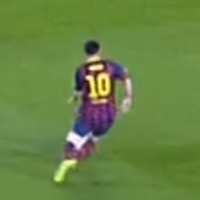
\includegraphics[width=.4\linewidth]{./images/resize_barcelona2.png}
        \captionof{figure}{En la imagen se observa la falta de resolución. Los
        bordes se ven difusos.
        \label{fig:barsa3}}
    \end{minipage}%
    \begin{minipage}[t]{.5\textwidth}
        \centering
        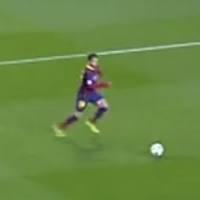
\includegraphics[width=.4\linewidth]{./images/resize_barcelona3.png}
        \captionof{figure}{Se observan dos de las dificultades del
        problema: la baja resolución y el diminuto tamaño de la pelota con
        respecto al jugador. \label{fig:barsa4}}
    \end{minipage}
\end{figure}

\subsection{Complejidad del Análisis en Tiempo Real}

Al tener una resolución de \textit{1080p} (aproximadamente dos millones de
píxeles por cuadro), el procesamiento de cada píxel debe tomar a lo sumo 20
nanosegundos. Para lidiar con esta restricción se puede utilizar información
adicional de la que se disponga respecto al video con el objeto de evitar
procesar píxeles de poca o nula utilidad para el seguimiento. Un ejemplo de
esto es descartar píxeles que estén fuera de la cancha, ya que es probable que
la cámara encuadre más que el campo de juego, abarcando las gradas, el público
espectador, publicidades alrededor del campo de juego, entre otros.

Muchos autores han desarrollado algoritmos automáticos de seguimiento de
objetos en secuencias de imágenes (ver \cite{IFTrace, alp, local-learning,
MHT-2}). Todos ellos están basados en soluciones de ecuaciones diferenciales en
derivadas parciales y proveen resultados precisos, pero tienen severas
restricciones que impiden que se utilicen para aplicaciones en tiempo real.

Para este trabajo, se utiliza el algoritmo de contornos activos (ver
\cite{fast-level-set}), el cual no utiliza ecuaciones diferenciales (haciéndolo
apto para aplicaciones en tiempo real) y además hace un análisis local de los
objetos seguidos en la imagen, lo cual hace que el tiempo de análisis de un
cuadro sea dependiente de la cantidad de píxeles que abarque la silueta de un
jugador e independiente del tamaño de cada cuadro del video.

\subsection{Distorsión de la Lente}

Al utilizar una única cámara para captar la cancha entera se corre el riesgo de
que los puntos de la imagen más alejados al foco de la cámara sufran una
distorsión. Este es el llamado ``efecto de ojo de buey'' e introduce mucho
error, por ejemplo en la aplicación de la homografía, por lo tanto se debe
aplicar una corrección. Una lente apropiada y bien calibrada puede reducir este
error, pero nunca puede ser eliminado totalmente. La Figura
\ref{fig:sin-correccion} muestra un cuadro con el efecto de distorsión y la
Figura \ref{fig:con-correccion} muestra el mismo cuadr, pero con la corrección
por software aplicada.

\begin{figure}[H]
    \centering
    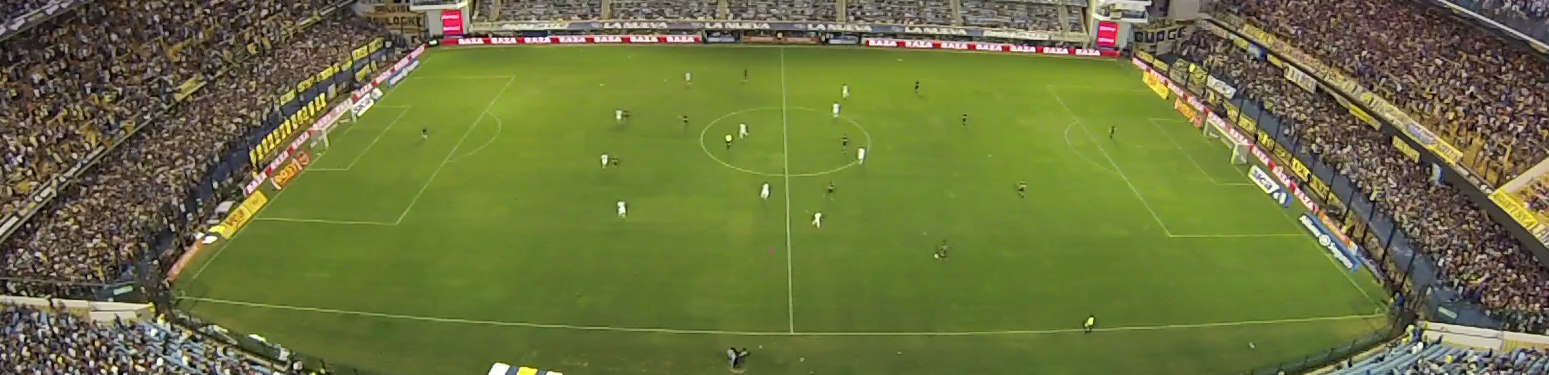
\includegraphics[width=.8\linewidth]{./images/sin-correccion.png}
    \captionof{figure}{Imagen afectada por distorsión de lente}
    \label{fig:sin-correccion}
\begin{figure}[H]
\end{figure}
    \centering
    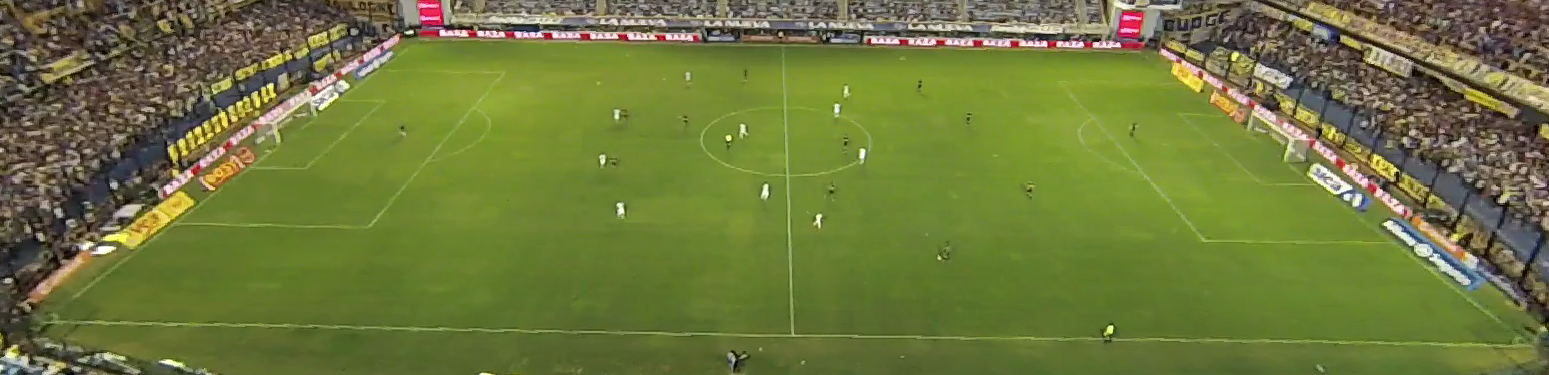
\includegraphics[width=.8\linewidth]{./images/con-correccion.png}
    \captionof{figure}{Misma imagen, con una corrección por software aplicada}
    \label{fig:con-correccion}
\end{figure}

% TODO: No explicamos un carajo como arreglamos esto

\subsection{Oclusiones entre Jugadores}

En un partido es muy común que los jugadores se crucen entre sí, ocultándose
parcial o totalmente de la cámara, y por lo tanto ocurran oclusiones entre los
jugadores. El sistema debe poder tolerar la oclusión parcial o total de los jugadores.
Esto puede llevar a situaciones muy difíciles de detectar automáticamente. Por
ejemplo, una situación particularmente difícil de resolver se dá cuando dos
jugadores del mismo equipo (con vestimenta muy similar) se encuentren alineados
con respecto a la cámara. Una posible solución es utilizar información de
cuadros anteriores para estimar la velocidad de cada uno y estimar sus nuevas
posiciones, pero esto es poco efectivo si los jugadores cambian de velocidad
mientras uno ocluye al otro, o si la velocidad era muy similar al momento de
generarse la oclusión.

Una situación problemática similar es una jugada de tiro de esquina (córner),
donde las oclusiones entre varios jugadores son muy numerosas, lo que agrega a
la restricción de tiempo real mayor complejidad, ya que la resolución de
oclusiones debe ser muy eficiente en tiempo.

